\documentclass[8pt,a4paper,compress,handout]{beamer}

\usepackage{/home/siyer/lib/slides}

\title{Defining Functions}
\date{}

\begin{document}
\begin{frame}
\vfill
\titlepage
\end{frame}

\begin{frame}
\frametitle{Outline}
\tableofcontents
\end{frame}

\section{.}
\begin{frame}[fragile]
\begin{framed}
\tiny harmonicf.py:  Write to standard output the harmonic numbers specified as command-line arguments.
\end{framed}

\begin{lstlisting}[language=Python]
import stdio
import sys

def harmonic(n):
    total = 0.0
    for i in range(1, n + 1):
        total += 1.0 / float(i)
    return total

def main():
    for j in range(1, len(sys.argv)):
        arg = int(sys.argv[j])
        value = harmonic(arg)
        stdio.writeln(value)

if __name__ == '__main__':
    main()
\end{lstlisting}

\begin{lstlisting}[language={}]
$ python harmonicf.py 1 2 4
1.0
1.5
2.08333333333
\end{lstlisting}
\end{frame}

\begin{frame}[fragile]
\begin{framed}
\tiny gauss.py: Accept floats $z$, $mu$, and $sigma$ as command-line arguments. Use them to test the Gaussian (normal) probability density (pdf) cumulative distribution (cdf) functions. Write the results to standard output.
\end{framed}

\begin{lstlisting}[language=Python]
import math
import stdio
import sys

def phi(x):
    return math.exp(- x * x / 2.0) / math.sqrt(2.0 * math.pi)

def pdf(x, mu = 0.0, sigma = 1.0):
    return phi((x - mu) / sigma) / sigma

def Phi(z):
    if z < -8.0:
        return 0.0
    if z > 8.0:
        return 1.0
    total = 0.0
    term = z
    i = 3
    while total != total + term:
        total += term
        term *= z * z / float(i)
        i += 2
    return 0.5 + phi(z) * total

def cdf(z, mu = 0.0, sigma = 1.0):
    return Phi((z - mu) / sigma)
\end{lstlisting}
\end{frame}

\begin{frame}[fragile]
\begin{lstlisting}[language=Python]
def main():
    z = float(sys.argv[1])
    mu = float(sys.argv[2])
    sigma = float(sys.argv[3])
    stdio.writeln(cdf(z, mu, sigma))

if __name__ == '__main__':
    main()
\end{lstlisting}

\begin{lstlisting}[language={}]
$ python gauss.py 820 1019 209
0.170509668691
$ python gauss.py 1500 1019 209
0.989316483738
$ python gauss.py 1500 1025 231
0.980122090737
\end{lstlisting}
\end{frame}

\begin{frame}[fragile]
\begin{framed}
\tiny coupon.py: Accept integer $n$ as a command-line argument. Write to standard output the number of coupons you collect before obtaining one of each of $n$ types.
\end{framed}

\begin{lstlisting}[language=Python]
import random
import stdarray
import stdio
import sys

def getCoupon(n):
    return random.randrange(0, n)

def collect(n):
    found = stdarray.create1D(n, False)
    couponCount = 0
    distinctCouponCount = 0
    while distinctCouponCount < n:
        coupon = getCoupon(n)
        couponCount += 1
        if not found[coupon]:
            distinctCouponCount += 1
            found[coupon] = True
    return couponCount

def main():
    n = int(sys.argv[1])
    couponCount = collect(n)
    stdio.writeln(couponCount)

if __name__ == '__main__':
    main()
\end{lstlisting}
\end{frame}

\begin{frame}[fragile]
\begin{lstlisting}[language={}]
$ python coupon.py 1000
5193
$ python coupon.py 1000
6865
$ python coupon.py 1000000
15490879
\end{lstlisting}
\end{frame}

\begin{frame}[fragile]
\begin{framed}
\tiny playthattunedeluxe.py: Read sound samples from standard input, add harmonics, and play the resulting sound to standard audio.
\end{framed}

\begin{lstlisting}[language=Python]
import math
import stdarray
import stdaudio
import stdio

def superpose(a, b, aWeight, bWeight):
    c = stdarray.create1D(len(a), 0.0)
    for i in range(len(a)):
        c[i] = a[i] * aWeight + b[i] * bWeight
    return c

def tone(hz, t):
    SPS = 44100
    n = int(SPS * t)
    a = stdarray.create1D(n + 1, 0.0)
    for i in range(n + 1):
        a[i] = math.sin(2.0 * math.pi * i * hz / SPS)
    return a

def note(pitch, t):
    CONCERT_A_HZ = 440.0
    NOTES_ON_SCALE = 12.0
    hz = CONCERT_A_HZ * (2.0 ** (pitch / NOTES_ON_SCALE))
    a = tone(hz, t)
    hi = tone(2 * hz, t)
    lo = tone(hz / 2, t)
    h = superpose(hi, lo, .5, .5)
    return superpose(a, h, .5, .5)
\end{lstlisting}
\end{frame}

\begin{frame}[fragile]
\begin{lstlisting}[language=Python]
def main():
    while not stdio.isEmpty():
        pitch = stdio.readInt()
        duration = stdio.readFloat()
        a = note(pitch, duration)
        stdaudio.playSamples(a)
    stdaudio.wait()

if __name__ == '__main__':
    main()
\end{lstlisting}

\begin{minipage}{170pt}
\begin{lstlisting}[language={}]
$ head -5 elise.txt
7 .125 
6 .125 
7 .125 
6 .125 
7 .125 
$ python playthattunedeluxe.py < elise.txt
\end{lstlisting}
\end{minipage}%
\begin{minipage}{130pt}
\hfill 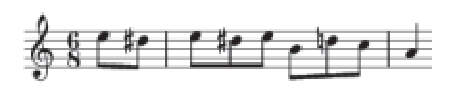
\includegraphics[scale=0.5]{figures/furelise.pdf}
\end{minipage}
\end{frame}
\end{document}
